\documentclass{standalone}
\usepackage{tikz}
\usetikzlibrary{calc,arrows}
\usetikzlibrary{decorations.pathreplacing,calligraphy}
\usepackage{pgfplots}
\usetikzlibrary{intersections, pgfplots.fillbetween}
\usetikzlibrary{snakes}
\usepackage{xcolor}

\begin{document}

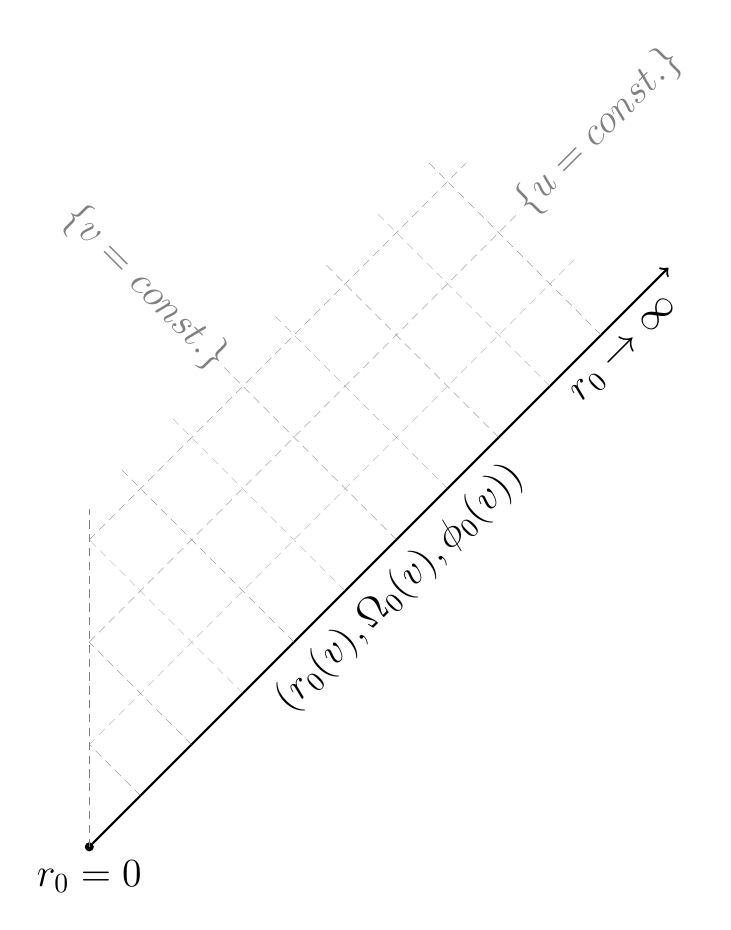
\begin{tikzpicture}[scale=1.3]

\node[circle, label= below:{\Large $r_0=0$}, draw,fill, inner sep =0, minimum size = .1cm] (n1) at (0,0) {};

\draw[thick, ->] (n1) -- (45:8);

\node[label= {[rotate=45]below:{\Large $\big(r_0(v), \Omega_0(v), \phi_0(v) \big)$}}] at (45:4) {};

\node[label= {[rotate=45]below:{ \Large$r_0 \rightarrow \infty $}}] at (45:7.2) {};

\draw[ultra thin, gray, densely dashed] (0,0) -- (0,3.3);
\draw[ultra thin, gray, densely dashed] (0,3) -- ($(0,3)+(45:5.2)$);

\draw[ultra thin, gray, densely dashed] (.5,.5) -- (0,1);
\draw[ultra thin, gray, densely dashed] (1,1) -- (0,2);
\draw[ultra thin, gray, densely dashed] (1.5,1.5) -- (0,3);
\draw[ultra thin, gray, densely dashed] (2,2) -- ($(2,2)+(135:2.4)$);
\draw[ultra thin, gray, densely dashed] (2.5,2.5) -- ($(2.5,2.5)+(135:2.4)$);
\draw[ultra thin, gray, densely dashed] (3,3) -- ($(3,3)+(135:2.4)$);
\draw[ultra thin, gray, densely dashed] (3.5,3.5) -- ($(3.5,3.5)+(135:2.4)$);
\draw[ultra thin, gray, densely dashed] (4,4) -- ($(4,4)+(135:2.4)$);
\draw[ultra thin, gray, densely dashed] (4.5,4.5) -- ($(4.5,4.5)+(135:2.4)$);
\draw[ultra thin, gray, densely dashed] (5,5) -- ($(5,5)+(135:2.4)$);

\draw[ultra thin, gray, densely dashed] (0,1) -- ($(0,1)+(45:6.7)$);
\draw[ultra thin, gray, densely dashed] (0,2) -- ($(0,2)+(45:5.9)$);

\node[label = {[rotate = 45 ,xshift = -1mm, yshift=1mm]right:	\color{gray}\Large $\{u =  const. \}$  }] at ($(0,2)+(45:5.9)$) {};

\node[label = {[rotate = -45 ,xshift = 1.8mm, yshift=1mm]left:	\color{gray} \Large$\{v =  const. \}$  }] at ($(3,3)+(135:2.4)$) {};  

\end{tikzpicture}

\end{document}